\chapter{Architecture of GRAPHINIUS}
\label{ch:graphinius_architecture}

\begin{figure}[ht]
	\label{fig_graphinius_architecture}
% \centering
% \includepdf[]{figures/Graphinius_Architecture}
\hspace*{-0.5cm}
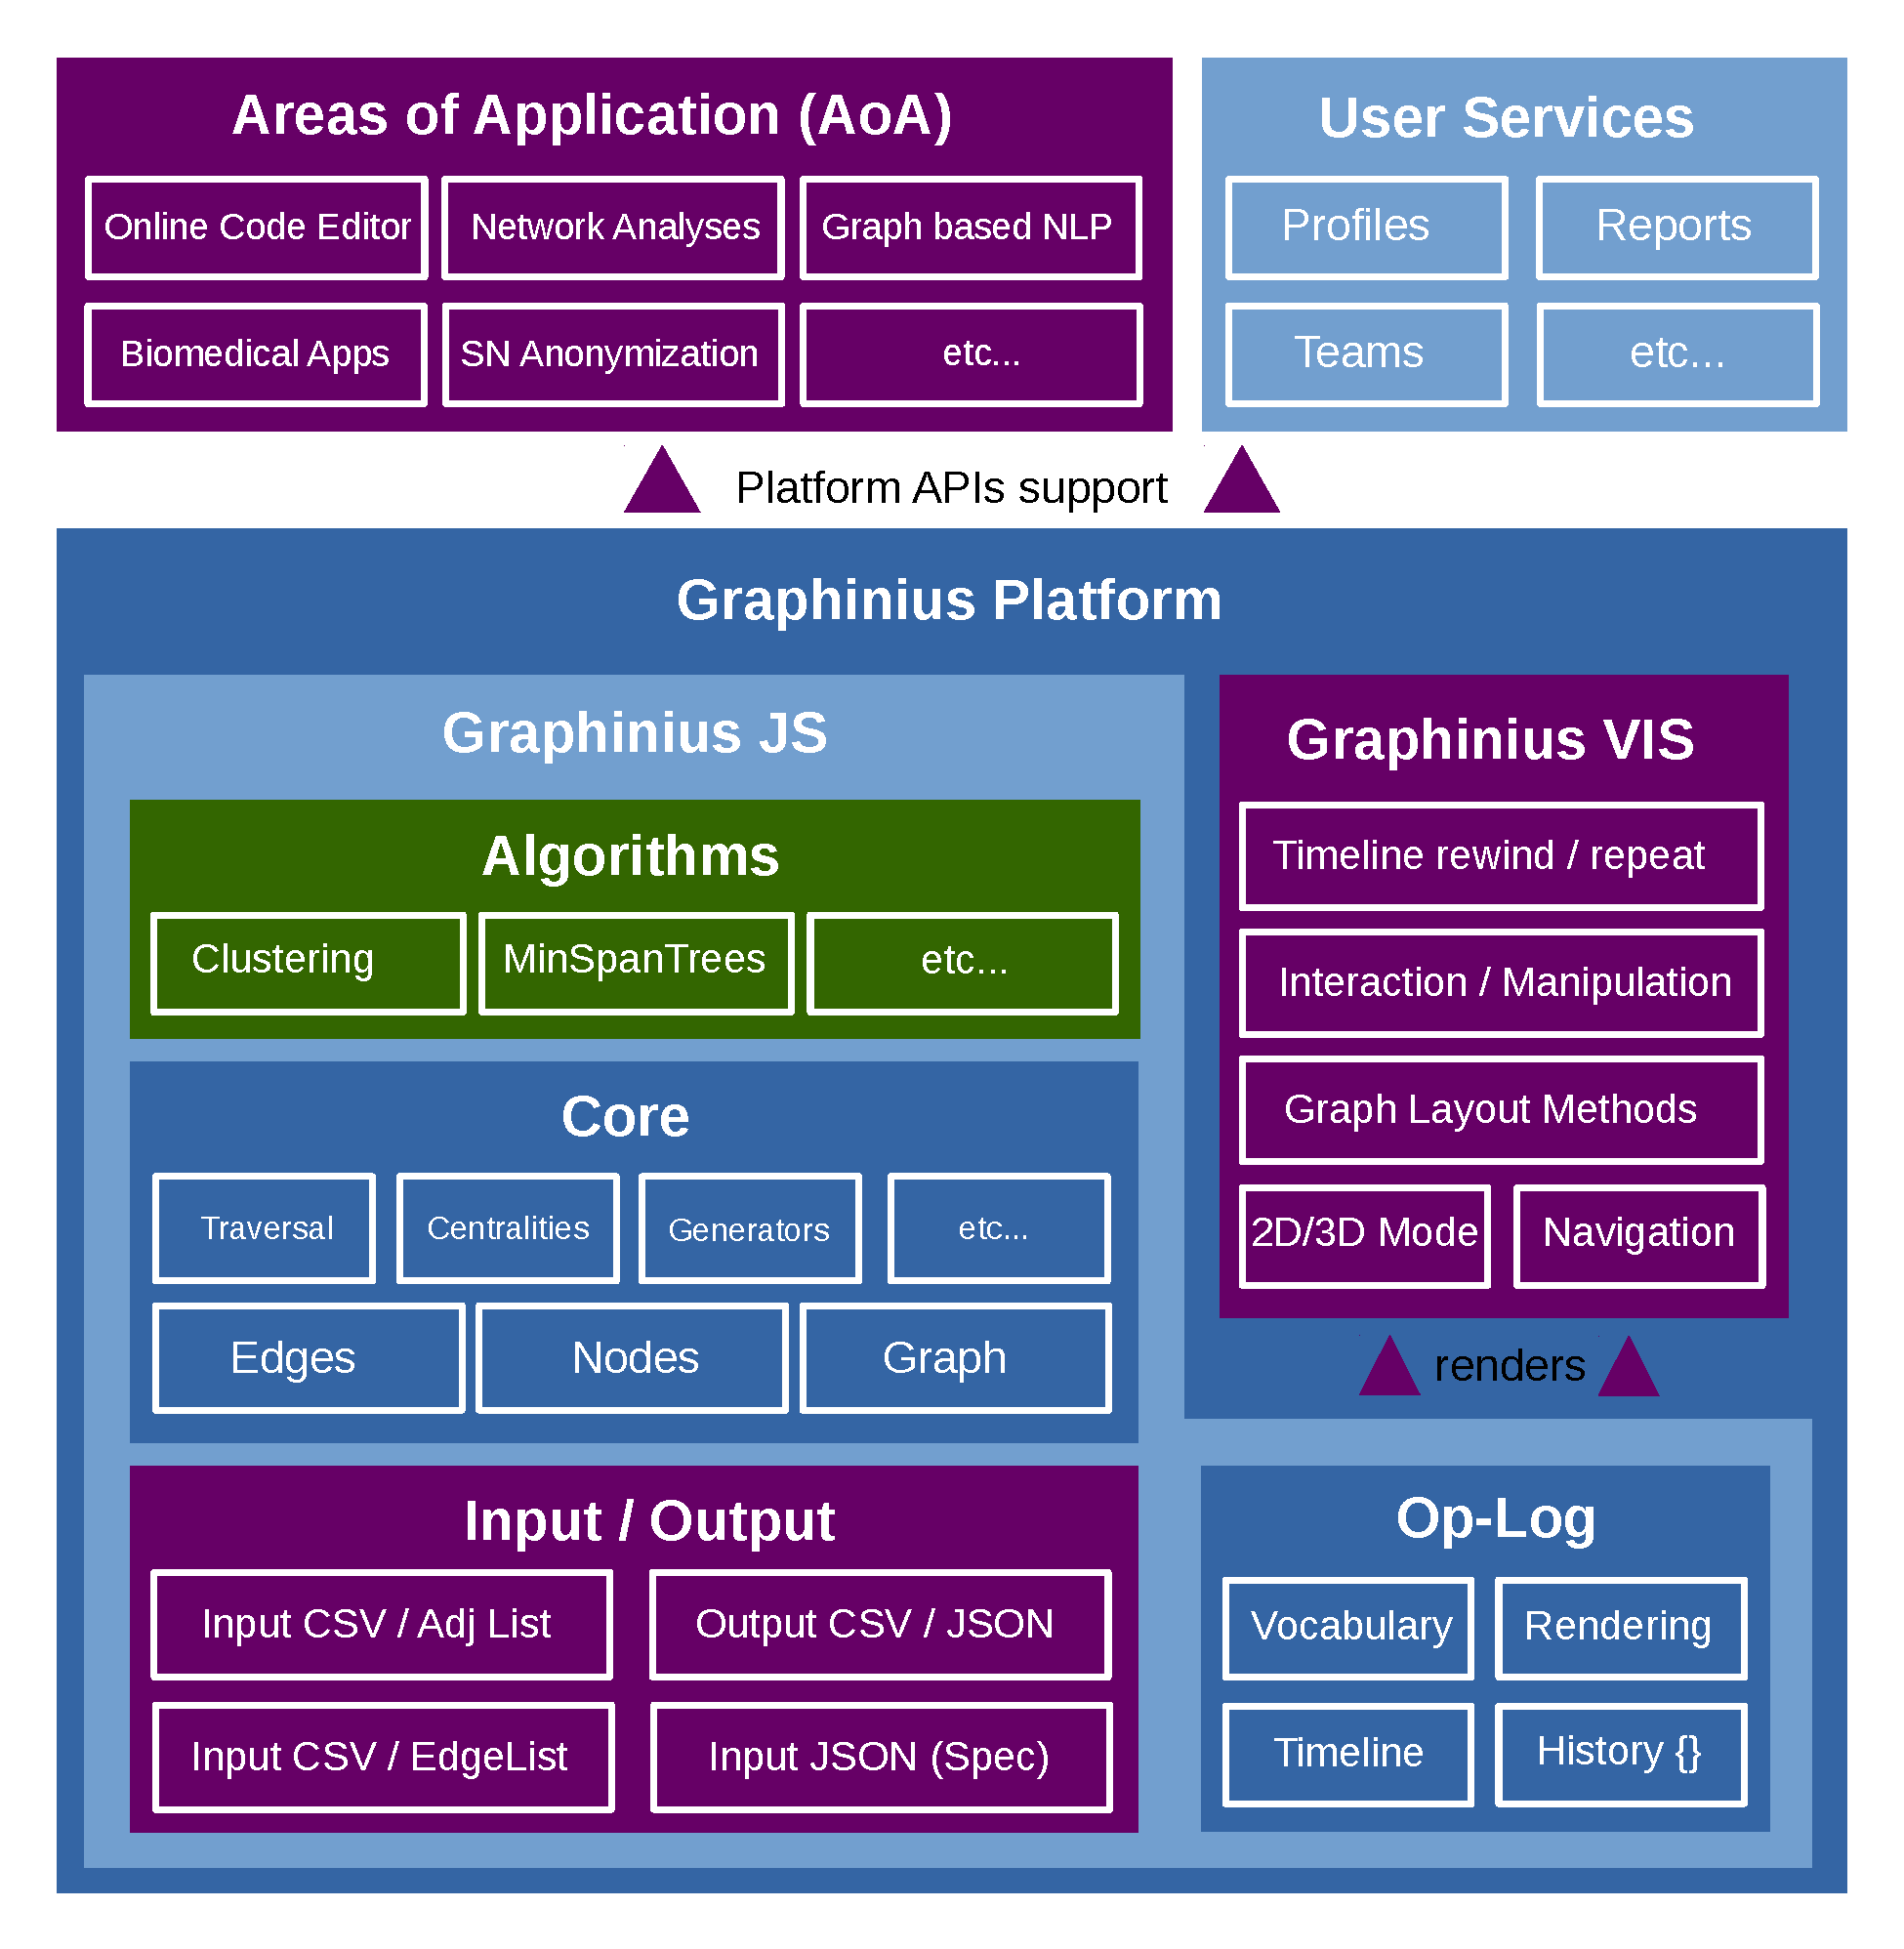
\includegraphics[width=1.1\textwidth]{figures/Graphinius_Architecture_pdf}
\end{figure}



\section{Graphinius Base}
\label{sect:graphinius_base}

As the name suggests, the Base offers all the functionality necessary to develop graph-based applications on top of it, including basic graph-computations and algorithms as well as visualization. It is therefore logically composed of those two modules, Graphinius JS and Graphinius VIS as well as a mechanism of communication between those two.
	

\section{Graphinius JS}
\label{sect:graphinius_js}

	\subsection{Input / Output}
	\label{ssect:input_output}
	
		\subsubsection{CSV}
		\label{sssection: io_csv}
		
		\subsubsection{JSON}
		\label{sssection: io_json}
	
	\subsection{Graph Core}
	\label{ssect:graph_core}
	
		\subsubsection{Edges}
		\label{sssection: core_edges}
		
		\subsubsection{Nodes}
		\label{sssection: core_nodes}
		
		\subsubsection{Graph}
		\label{sssection: core_graph}
		
		\subsubsection{Traversal}
		\label{sssection: core_traveral}
		
		BFS / DFS implementations... [figure: callback-based DFS]
		
		\subsubsection{Degrees}
		\label{sssection: core_degrees}
		
		\subsubsection{Centralities}
		\label{sssection: core_centralities}
		
		\subsubsection{Generators}
		\label{sssection: core_}
		
	
	\subsection{Algorithms}
	\label{ssect:algorithms}
	
		\subsubsection{Clustering}
		\label{sssection: algo_clustering}
		
		\subsubsection{MinSpanTrees}
		\label{sssection: algo_minspan}
		
		\subsubsection{Shortest Paths}
		\label{sssection: algo_shorest_paths}


\section{The Op-Log}
\label{sect:op_log}

	\subsection{Timeline}
	\label{ssect:timeline}
	
	\subsection{History Object}
	\label{ssect:history_object}

	\subsection{Vocabulary}
	\label{ssect:vocabulary}	

	\subsection{Rendering Mechanism}
	\label{ssect:rendering}


\section{Graphinius VIS}
\label{sect:graphinius_vis}

	\subsection{2D/3D Mode}
	\label{ssect:vis_2d3d}
	
	\subsection{Navigation}
	\label{ssect:vis_navigation}
	
	\subsection{Graph Layouts}
	\label{ssect:vis_layouts}	
	
	\subsection{Interaction / Manipulation}
	\label{ssect:vis_interact_manipulate}
	
	\subsection{Timeline rewind / repeat}
	\label{ssect:vis_timeline}


\begin{landscape}
\begin{figure}[ht]
	\label{fig_history_workflow}
	\centering
	\vspace{-2.0cm}
%	\hspace*{0cm}
	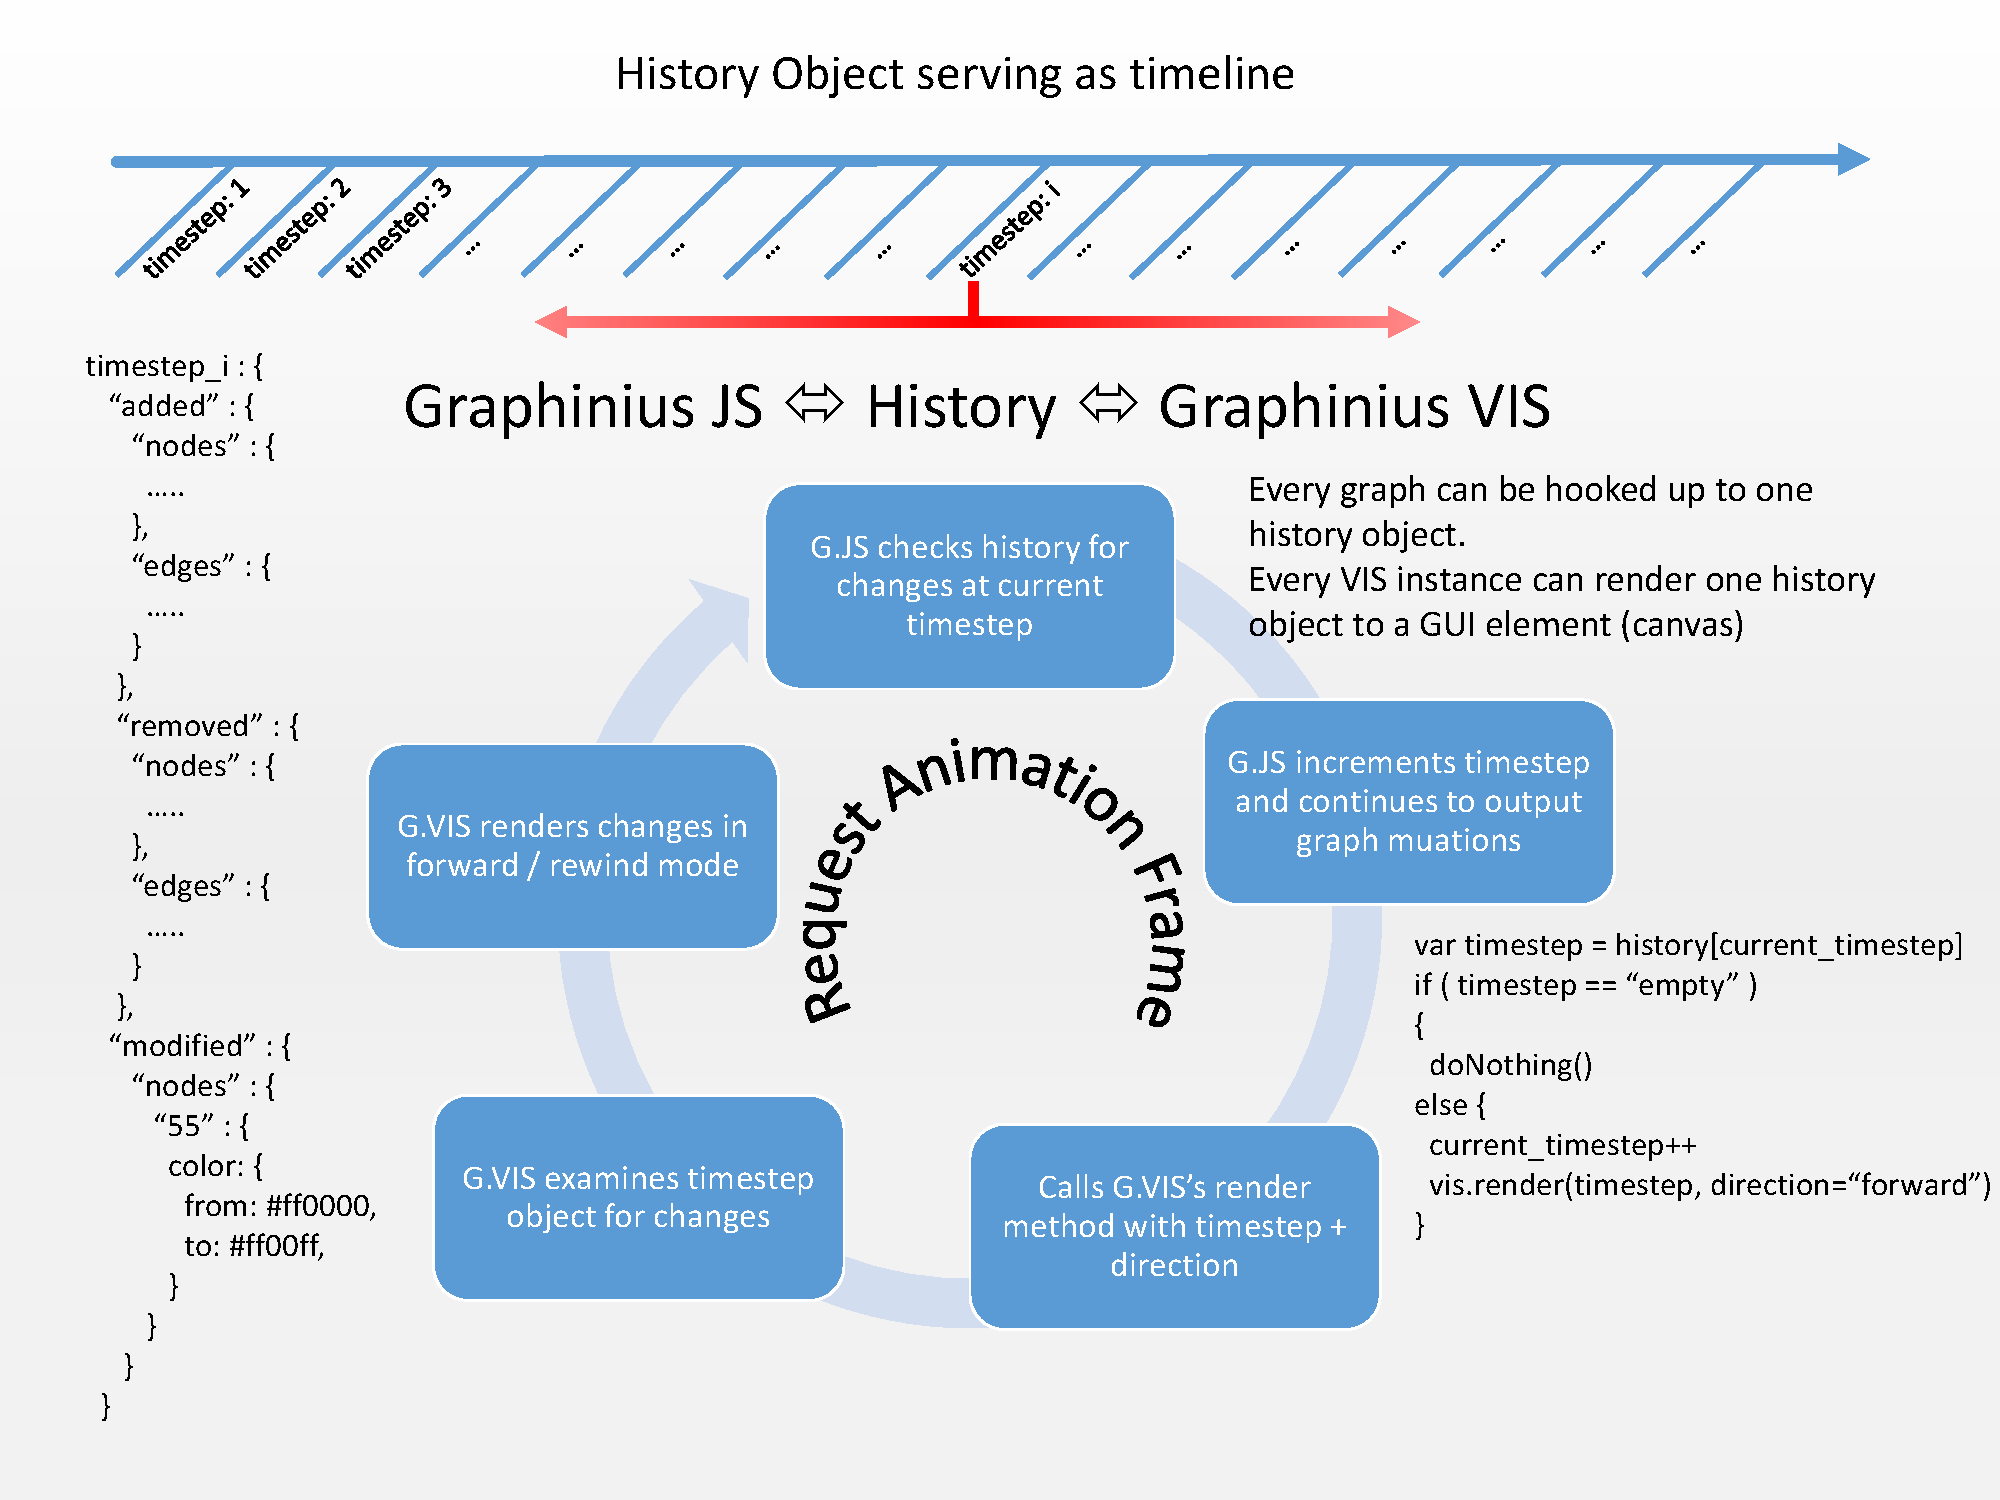
\includegraphics[width=1.7\textwidth]{figures/History_Workflow_pdf}
\end{figure}
\end{landscape}



\section{Areas of Applications (AoA)}
\label{sect:areas_of_applications}

	\subsection{Online Editor}
	\label{ssect:aoa_editor}
	
	\subsection{Biomedical Applications}
	\label{ssect:aoa_bioapps}
	
	\subsection{SN Anonymization}
	\label{ssect:aoa_anonym}


\section{Platform Services}
\label{sect:platform_services}

	\subsection{Personal Profile}
	\label{ssect:service_profile}
	
	\subsection{Teams}
	\label{ssect:service_teams}
	
	\subsection{Output / Reports}
	\label{ssect:service_output}